% Template for a Computer Science Tripos Part II project dissertation
\documentclass[12pt,a4paper,twoside,openright]{report}
\usepackage[pdfborder={0 0 0}]{hyperref}    % turns references into hyperlinks
\usepackage[margin=25mm]{geometry}  % adjusts page layout
\usepackage[export]{adjustbox}
\usepackage{graphicx}  % allows inclusion of PDF, PNG and JPG images
\usepackage{verbatim}
\usepackage{docmute}   % only needed to allow inclusion of proposal.tex

\graphicspath{ {Images/} }
\raggedbottom                           % try to avoid widows and orphans
\sloppy
\clubpenalty1000%
\widowpenalty1000%

\renewcommand{\baselinestretch}{1.1}    % adjust line spacing to make
                                        % more readable

\begin{document}

%%%%%%%%%%%%%%%%%%%%%%%%%%%%%%%%%%%%%%%%%%%%%%%%%%%%%%%%%%%%%%%%%%%%%%%%
% Title


\pagestyle{empty}

\rightline{\LARGE \textbf{George Andersen}}

\vspace*{60mm}
\begin{center}
\Huge
\textbf{QWOP in JavaScript} \\[5mm]
Computer Science Tripos -- Part II \\[5mm]
Robinson College \\[5mm]
\today  % today's date
\end{center}

% \vspace{5mm}

% \newpage
% \section*{Declaration}

% I, George Andersen of Robinson college being a candidate for Part II of the Computer Science Tripos, hereby declare that this dissertation and the work described in it are my own work, unaided except as may be specified below, and that the dissertation does not contain material that has already been used to any substantial extent for a comparable purpose.

% \bigskip
% \leftline{Signed George Andersen}

% \medskip
% \leftline{Date \today}

% %%%%%%%%%%%%%%%%%%%%%%%%%%%%%%%%%%%%%%%%%%%%%%%%%%%%%%%%%%%%%%%%%%%%
% % Introduction (intro+prep ~3000)
% \chapter{Introduction}
% \section{section 1}
% introduction



% %%%%%%%%%%%%%%%%%%%%%%%%%%%%%%%%%%%%%%%%%%%%%%%%%%%%%%%%%%%%%%%%%%%%
% % Preparation (intro+prep ~3000)
% \chapter{Preparation}
% \section{section 1}
% Preparation

% In this chapter, I have discussed the theory that had to be understood, and work that
% had to be done, before implementation could begin




%%%%%%%%%%%%%%%%%%%%%%%%%%%%%%%%%%%%%%%%%%%%%%%%%%%%%%%%%%%%%%%%%%%%
% Implementation ~4500
\chapter{Implementation}

This chapter describes the implementation of the project, moving on from preparation in previous chapters. The main implementation tasks in the project were writing my version of QWOP, and writing the set of software used to perform the user study and evaluate the project. These can be divided as follows:

\begin{enumerate}
  \item Phaser Implementation of QWOP
	\begin{enumerate}
      \item Modelling joints in physics
  	  \item Modelling the athlete
  	  \item Graphics
  	  \item Game flow
	\end{enumerate}
  \item Evaluation software
    \begin{enumerate}
      \item Web page hosting user study
      \item Server software to receive and store user study data
      \item Chrome extension for reading distance from QWOP
    \end{enumerate}
\end{enumerate}

\section{Phaser Implementation of QWOP}

Phaser is a JavaScript framework designed for making games. I have described how it works in the preparation section, and will now break down how it was used to make the different sections of the game.


\begin{enumerate}
	\item Modelling joints in physics

	The first hurdle was to work out how to create a body in Phaser's physics engine.   
	\ref{swingingRods} shows my first prototype for modelling joints and limbs, each rod is a sprite, and the joints between them are fixed together by Phaser's 'revoluteContraint's. This allows them to swing freely.

	\begin{figure}[tbh]
	\centerline{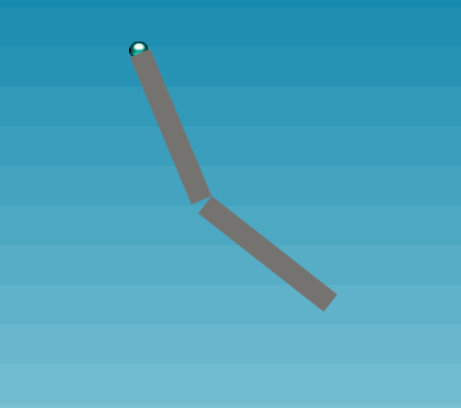
\includegraphics[scale=0.5]{swingingRods.PNG}}
	\caption{Swinging rods initial model of limbs}
	\label{swingingRods}
	\end{figure}

	The next step was make the joints apply forces to each other. This would be used to not only move the limbs when the user presses the keys, but also provide forces so that the body would stay in a similar position when keys are not pressed.

	The way I did this was to use Phaser's motors on the joints. These work by applying the force needed to move the joint at the specified speed, capped off at a max value. This way of powering joints could also be used easily to apply the static forces by setting the speed to 0.

	%%%%%%%%%%%%%%%%%%%%%%%%%%%%%%%%%%%%%%%%%%%%%%%%%%%%%%%%%%%%%%%%%%%
	% Older versions

	% https://cdn.rawgit.com/gla23/Part2Project/b43f453d1597b3f8080149ee5ca01760d64828dc/QWOPjs.html
	% swinging rods

	% https://cdn.rawgit.com/gla23/Part2Project/2b6292ed7cc0cb4994fea7af4697a1c1091b484d/QWOPjs.html
	% 1 leg 
	
	% https://cdn.rawgit.com/gla23/Part2Project/90935e3f9d1c2ff3d96cb271449743c98e651588/QWOPjs.html
	% body without graphics

	%https://cdn.rawgit.com/gla23/Part2Project/a76f298dcf66717188357c85e1b0b7667cea8e46/myQWOPjs.html
	% with graphics

	\item Modelling the athlete

	To model the athlete from these sprite joints, I specified the dimensions, mass, offset and starting rotation of each limb. Then forward kinematics is used on this data to get the starting points of the limbs. The limbs are then instantiated in these starting positions with the correct mass, dimensions and 'revoluteConstraint' joints. 
	These joints are given joint limits so that each limb has a realistic range of motion, for example the knee joint doesn't let your lower leg rotate all the way round.
	The motors for these joints are then attached to the user input according to the control scheme. If a key is pressed that powers the limb, the motor is set to the limb power, otherwise it is set to 0 so that the static forces apply.

	Each limb is given a group so that materials 
	either part of the  or  group, that 
	
	\begin{figure}[tbh]
	\centerline{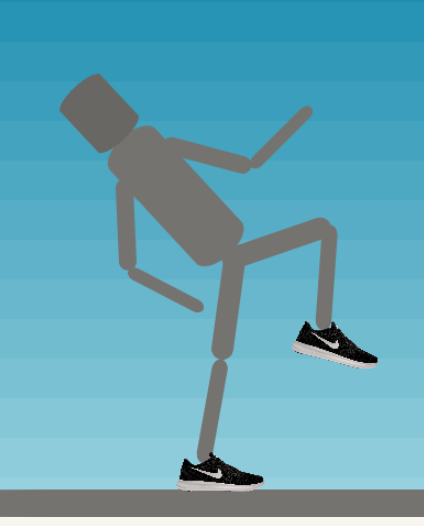
\includegraphics[scale=0.5]{athleteModel.PNG}}
	\caption{model of athlete}
	\label{athleteModel}
	\end{figure}

	\item Graphics

	Next the graphics were added to the model so that it looked similar to the original QWOP.
	Each sprite was given an image taken from the original.

	\begin{figure}[tbh]
	\centerline{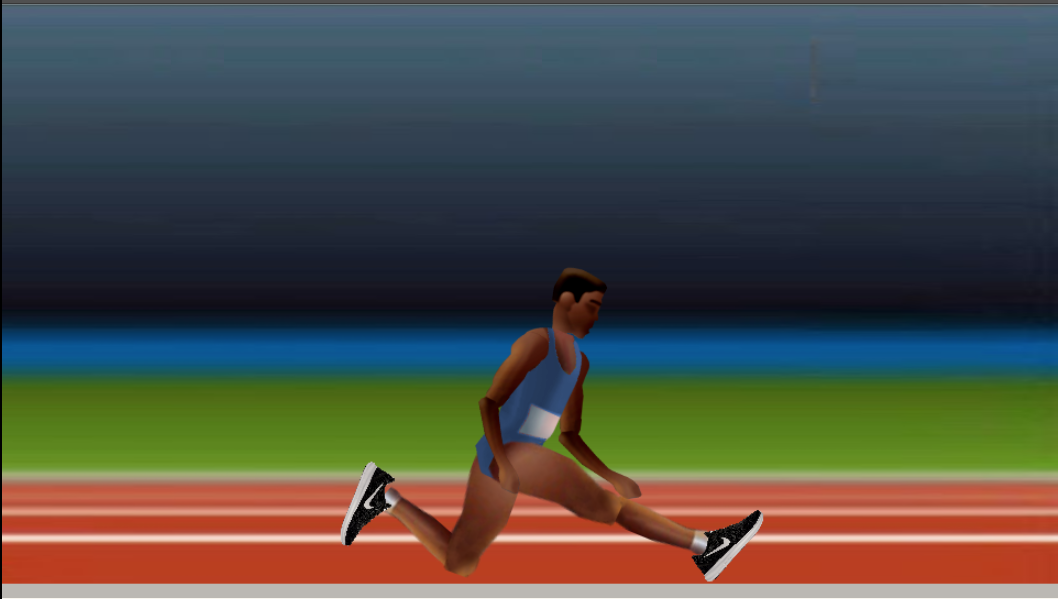
\includegraphics[scale=0.4]{Images/modelWithGraphics.PNG}}
	\caption{model with graphics added}
	\label{modelWithGraphics}
	\end{figure}

	\item Game flow

	Finally all the other components of the game were added:

	\begin{enumerate}
		\item Collisions with the floor - Each limb that cannot touch the floor is put into a collision group. This group is used to check whether a collision with the floor occurs, and if so end the game.
		\item Calculation of distance reached so far - a function of the x value of the athletes torso
		\item Text showing the distance reached on the screen.
		\item Recording the high score and displaying it on the screen
		\item A User help box shown on game start-up
		\item Checking whether the user has reached the end of the 100m and displaying the congratulations message if the player gets to 100m
	\end{enumerate}
\end{enumerate}

\section{Evaluation software}

To evaluate the project, I will be analysing the results from a user study. This analysis will be happening in the evaluation section, however a large amount of work went into implementing the testing environment so I will describe that here.

% breakdown of user study sections used later
\newcommand{\userStudySections}{
	\begin{enumerate}
		\item A html page that guides the participant through the sections of the study
		\item An embedded Google form that finds out demographics and the previous experience of each participant.
		\item An A/B test. Each participant is randomly placed into one of the two groups, each of which play the two versions of QWOP in a different order. Each game is played for 5 minutes before the page moves onto the next section. While each game is played, the key presses and distances reached for each participant are recorded. The benefit of doing a randomised control trial is that selection bias is minimised. The splitting of participants into two groups means that the effect of playing one game before the other can be taken into consideration and not affect the analysis.
		\item A final questionnaire that gives feedback on the two versions
	\end{enumerate}
}

\begin{enumerate}
	\item Web page hosting user study

	As I wanted to get lots of participants to take part in my user study, I decided to host it on a web page so that participants can take part concurrently. It was also useful as I can host both versions of QWOP in iframes, embed Google forms as questionnaires, and record the actions of the user. The actions of the user such as key presses and distances reached over time can be analysed along with other data to evaluate the success of the game.

	The main components of the web page are as follows:

	\userStudySections

    \item Server software to receive and store user study data

    I hosted the web page page on my SRCF web space. When the web page is recording data, it sends the data it has recorded to a PHP script at regular time intervals. This script records the data into separate files for each participant, so that all the data can be accessed in one place afterwards.

    \item Chrome extension for reading distance from QWOP

    Later on in the implementation I discovered that I couldn't access the distance that the player had reached for the original QWOP. It it impossible to access data from the game when hosting the original website inside an iframe, since all the game data is inside an anonymous function.
    Unfortunately When attempting to run the game by taking the html, JavaScript and other local resources that it accessed, and running them myself, the game's canvas goes orange and the game doesn't start.
    Since running an edited version of the original website did not work, I tried accessing the colour values of the game's canvas, then I could use OCR to read the distance from the screen itself. Accessing the pixel values from the canvas inside the iframe didn't work as QWOP has a OpenGL setting that made the GLBuffer unreadable.s
    In the end however the distance was made accessible by creating a chrome extension that took a screenshot of the page and placed it in a canvas. Then the data collection page takes the section of the screenshot that contains the distance text, inverts the colours so that it's black text on a white background, and places it into a smaller canvas. Then a lightweight JavaScript OCR script called ocrad.js is used to to read the text. With a little editing of the script's output, it gave an accurate value.
\end{enumerate}



% %%%%%%%%%%%%%%%%%%%%%%%%%%%%%%%%%%%%%%%%%%%%%%%%%%%%%%%%%%%%%%%%%%%%
% % Evaluation (eval+conc ~ 2500)
\chapter{Evaluation}
\section{success criteria?}

\section{User Study}
To evaluate the project I have performed a user study.
The user study is made up of these sections, the design on which has been discussed in the implementation:

\userStudySections

\section{Participant demographics}

30 participants took part in the user study. This is a good number because...


The first questionnaire asked for the demographics of each participant. Figure \ref{demographics} shows the age and gender of the participants.

\begin{figure}[tbh]
\centerline{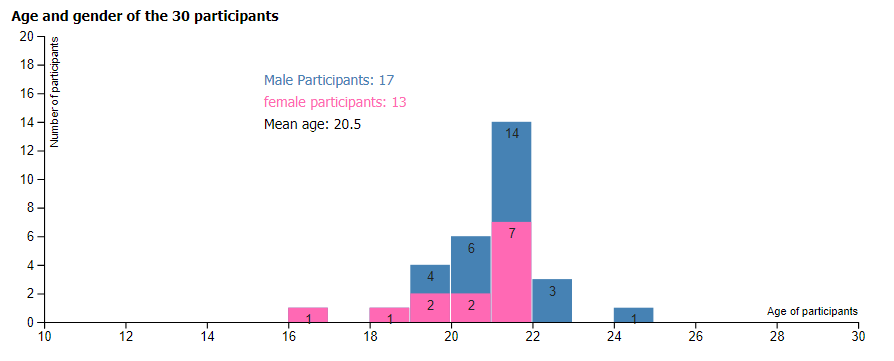
\includegraphics[scale=0.5]{participantDemographics.PNG}}
\caption{Participant demographics}
\label{demographics}
\end{figure}

The next question asked was whether the user had played QWOP beforehand. Here are the results:


\begin{tabular}{ |c|c| }
  \hline
  Previous experience playing QWOP & Frequency of choice \\ \hline \hline 
  A long time over multiple sessions & 1 \\ \hline
  Longer than 30 minutes & 2 \\ \hline
  Between 10 and 30 minutes & 3 \\ \hline
  Less than 10 minutes & 5 \\ \hline
  Never played before & 19 \\
  \hline
\end{tabular}

Most of the user hadn't played QWOP before.

it effects it like ???


% %%%%%%%%%%%%%%%%%%%%%%%%%%%%%%%%%%%%%%%%%%%%%%%%%%%%%%%%%%%%%%%%%%%%
% % Conclusion (eval+conc ~ 2500)
% \chapter{Conclusion}
% \section{section 1}
% Conclusion





\end{document}
